 

Els recollidors de memòria brossa (\textit{garbage collectors} en anglès) son un mecanisme propi d'alguns llenguatges de programació que, 
de forma transparent al programador, gestionen la memòria. Aquest mecanisme de gestió implicita de la memòria va ser dissenyat per primer 
cop per simplificar la gestió de memòria al llenguatge de programació LISP.

\par

Per una petita aproximació a aquets algoritmes, prenem com a model l'execucció d'un programa en C, representat a la figura \ref{fig:codiC}.
Podem veure com la memòria dinàmica d'un programa està gestionada a través de crides al sistema operatiu amb una interfície senzilla. 

\begin{figure}[h]
    \centering
    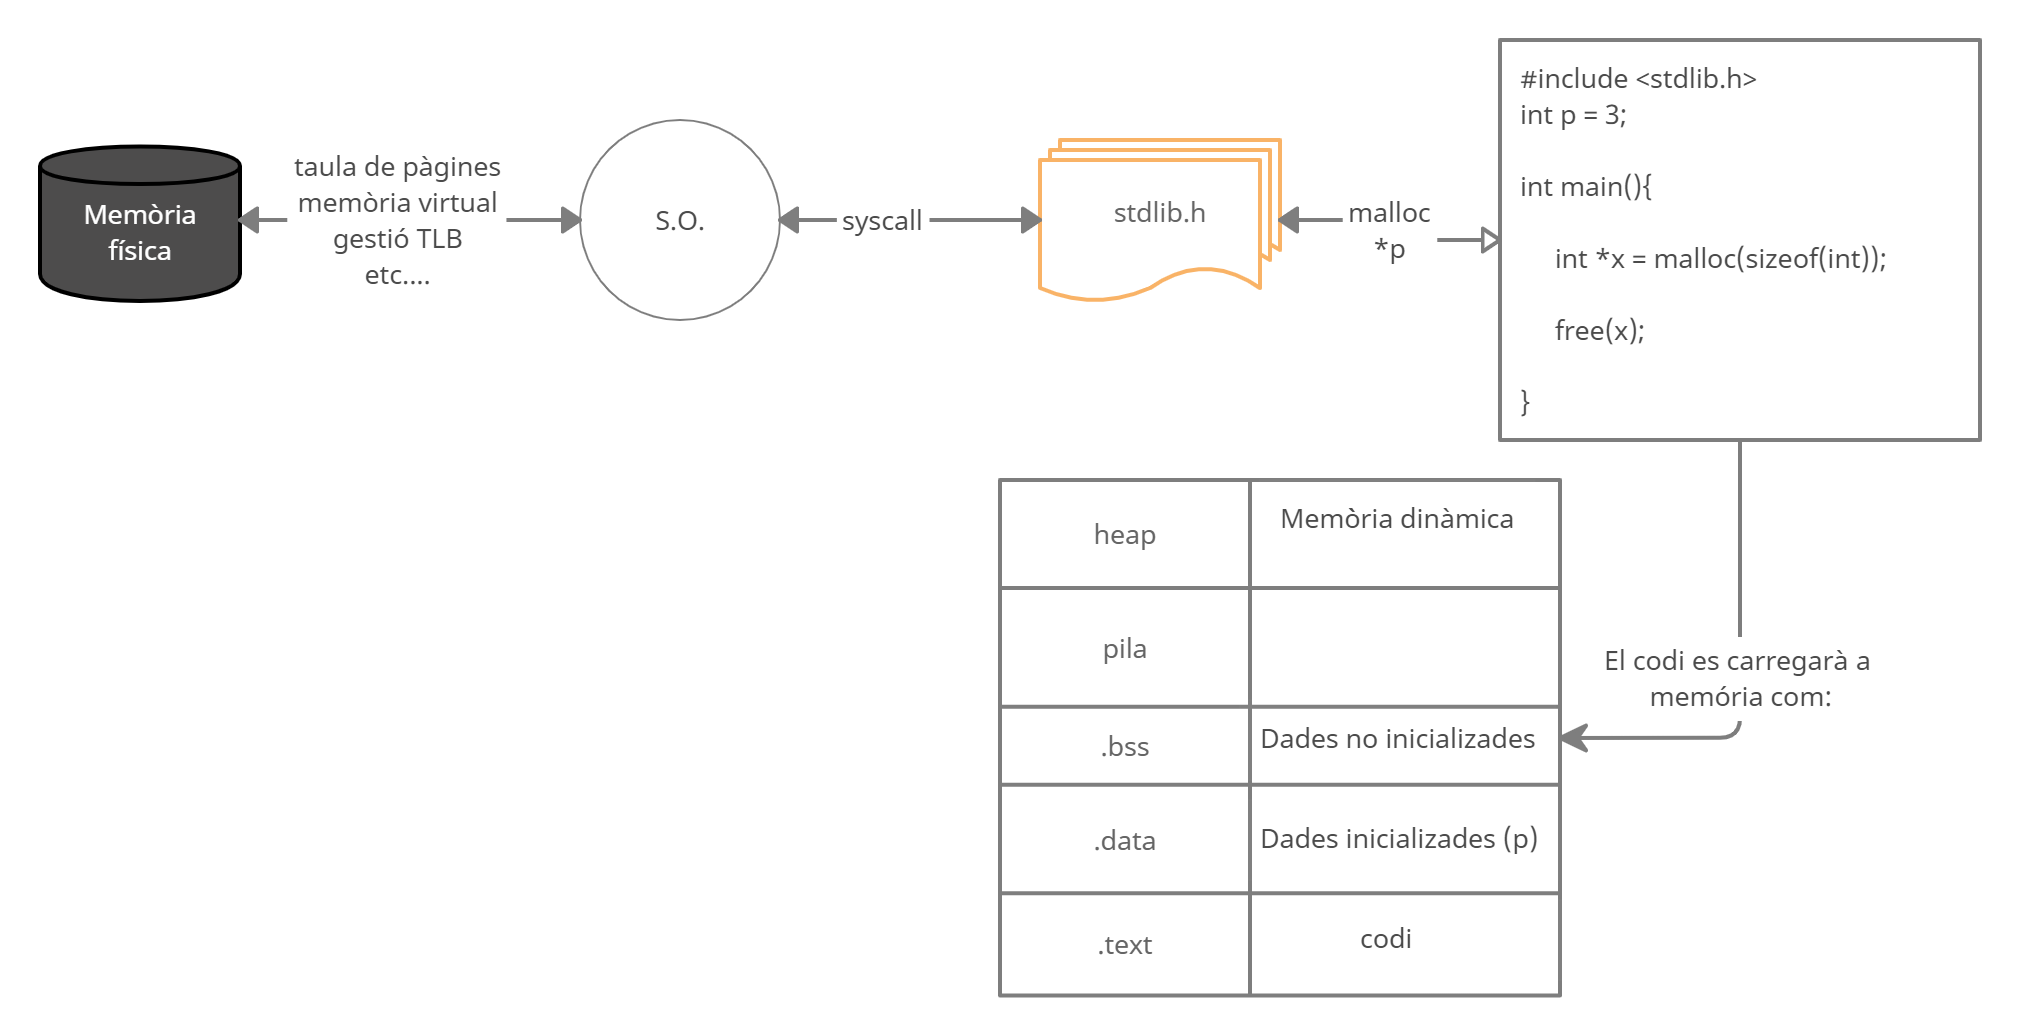
\includegraphics[width=\textwidth]{c_std_memory.png}
    \caption{Execucció d'un codi en C/C++}
    \label{fig:codiC}
\end{figure}

En un codi similar a aquets podem tenir errors en temps d'execucció, per exemple, si provem d'accedir al punter un cop s'ha alliberat. 
Errors similars, deguts a una mala programació, són els que ataquen els sistemes de recollida de memòria brossa.

\par
Com a contrapartida d'aquesta automatització de la gestió de la memòria, el rendiment pot veure's afectat, doncs
els GC no són un algoritme que s'executa alhora que el codi que s'ha programat. En aquest treball s'exposaran els errors que ens sol·lucionen aquets mecanismes.

